\documentclass[12pt, titlepage]{article}

\usepackage{pdflscape}
\usepackage{fullpage}
\usepackage[round]{natbib}
\usepackage{multirow}
\usepackage{booktabs}
\usepackage{tabularx}
\usepackage{graphicx}
\usepackage{float}
\usepackage{hyperref}
\hypersetup{
    colorlinks,
    citecolor=blue,
    filecolor=black,
    linkcolor=red,
    urlcolor=blue
}

%% Comments

\usepackage{color}

\newif\ifcomments\commentstrue %displays comments
%\newif\ifcomments\commentsfalse %so that comments do not display

\ifcomments
\newcommand{\authornote}[3]{\textcolor{#1}{[#3 ---#2]}}
\newcommand{\todo}[1]{\textcolor{red}{[TODO: #1]}}
\else
\newcommand{\authornote}[3]{}
\newcommand{\todo}[1]{}
\fi

\newcommand{\wss}[1]{\authornote{blue}{SS}{#1}} 
\newcommand{\plt}[1]{\authornote{magenta}{TPLT}{#1}} %For explanation of the template
\newcommand{\an}[1]{\authornote{cyan}{Author}{#1}}

%% Common Parts

\newcommand{\progname}{MTOBridge} % PUT YOUR PROGRAM NAME HERE
\newcommand{\authname}{Team 15, Alpha Software Solutions
\\ Badawy, Adham
\\ Yazdinia, Pedram
\\ Jandric, David
\\ Vakili, Farzad
\\ Vezina, Victor
\\ Chiu, Darren} % AUTHOR NAMES                  

\usepackage{hyperref}
    \hypersetup{colorlinks=true, linkcolor=blue, citecolor=blue, filecolor=blue,
                urlcolor=blue, unicode=false}
    \urlstyle{same}


\newcounter{acnum}
\newcommand{\actheacnum}{AC\theacnum}
\newcommand{\acref}[1]{AC\ref{#1}}

\newcounter{ucnum}
\newcommand{\uctheucnum}{UC\theucnum}
\newcommand{\uref}[1]{UC\ref{#1}}

\newcounter{mnum}
\newcommand{\mthemnum}{M\themnum}
\newcommand{\mref}[1]{M\ref{#1}}

\begin{document}

\title{System Design for \progname{}} 
\author{\authname}
\date{\today}

\maketitle

\pagenumbering{roman}

\section{Revision History}

\begin{tabularx}{\textwidth}{p{2.5cm}p{3.5cm}X}
\toprule {\bf Date} & {\bf Developer(s)} & {\bf Change}\\
\midrule
15/01/2023 & Farzad & Initial Draft\\
17/01/2023 & Victor & Added Timeline and Protocol Design\\
\bottomrule
\end{tabularx}

\newpage

\section{Reference Material}

This section records information for easy reference.

\subsection{Abbreviations and Acronyms}

\renewcommand{\arraystretch}{1.2}
\begin{tabular}{l l} 
  \toprule		
  \textbf{symbol} & \textbf{description}\\
  \midrule 
  \progname & Explanation of program name\\
  \wss{...} & \wss{...}\\
  \bottomrule
\end{tabular}\\

\newpage

\tableofcontents

\newpage

\listoftables

\listoffigures

\newpage

\pagenumbering{arabic}

\section{Introduction}
The following is a high level system design document for the MTOBridge software, a program for load rating bridges experiencing strain caused by self driving truck platoons. For more information on this software, you can consult the following documents as needed:\\
\href{../../SRS/SRS.pdf}{Link to SRS}\\
\href{../../HazardAnalysis/HazardAnalysis.pdf}{Link to HA}\\
\href{../../VnVPlan/VnVPlan.pdf}{Link to V\&V}\\
\href{../../Design/SoftArchitecture/MG.pdf}{Link to MG}\\
\href{../../Design/SystDesign/SystDes.pdf}{Link to MIS}\\
\section{Purpose}
This document is intended to provide a high-level view of the design decisions made with regards to the user interface component of the MTOBridge software, along with a planned timeline of implementation.

\section{Scope}
Note that this document, as well as all others written by this team, will focus purely on the visualization and user interface component of MTOBridge, ignoring the backend MATLAB solvers as this component will not be designed by this team, nor does this team have any hand in that design. A simple diagram outlining the system boundaries can be found below.
\begin{figure}[H]
  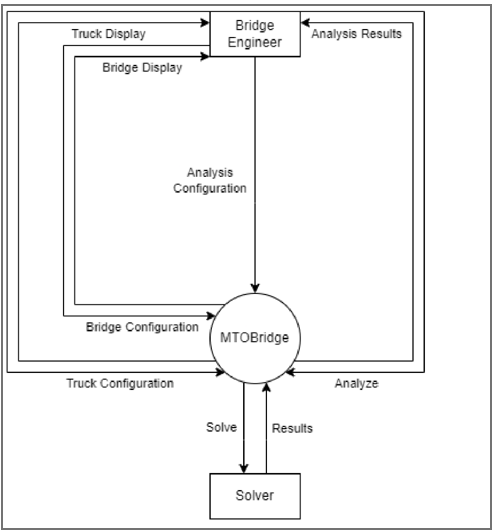
\includegraphics[]{../images/system-boundaries.PNG}
  \caption{System Boundaries Diagram}
  \label{fig:system-boundaries-diagram}
\end{figure}

\section{Project Overview}

\subsection{Normal Behaviour}
Assuming everything goes smoothly, the most general user scenario for MTOBridge is as follows:\\
\begin{enumerate}
\item A user launches the program
\item They set up/load a truck platoon configuration
    \begin{itemize}
        \item [2a.] They may choose to save their configuration for later
    \end{itemize}
\item They set up/load a bridge configuration
    \begin{itemize}
        \item [3a.] They may choose to save their configuration for later
    \end{itemize}
\item They set up/load a solver configuration
    \begin{itemize}
        \item [4a.] They may choose to save their configuration for later
    \end{itemize}
\item They run the calculations
\item A visualization of the results is presented to them
\item The output report is created and shown to them
\item The out report is saved to the file system
    \begin{itemize}
        \item [8a.] They may choose to return to step 1
    \end{itemize}
\item They exit the program
\end{enumerate}
\subsection{Undesired Event Handling}
As this is a user interface, robustness and reliability are of the utmost importance for a good user experience. Crashes, slowdowns, or hangs as a result of unexpected events will be highly detrimental to the quality of the program. With this in mind, the plan is to attempt to foresee and catch as many different types of errors as possible, and otherwise allow the program to fail in a palatable way. For example, if during step 4 the user inputs an invalid bridge configuration (i.e choosing “swaws” as the length of their bridge), the program will be set up to prompt them to enter another length, as their current one is invalid and it needs to be a number between x and y, say.
Another consideration is to design the program in such a manner so as to limit the possibility of undesired events occurring, by removing user freedom. For example, only allowing users to drag a slider from x to y meters to determine the length of their bridge rather than having them type it in, or some other form of input where the range of inputs can be controlled. This can make the program feel constrained, but also create a safer runtime where the user is not given enough rope to hang themselves.
Which of these undesired event handling techniques is applied will depend on the context, something like user input is simple and its errors catchable enough that the first method seems feasible. However, the amount of interaction with the visualization/animation of the calculation results available to the user is a much less discrete design space, and therefore might have to be limited using the second method. The choice of method and its application will be refined through testing, both for robustness and quality of life.
\subsection{Component Diagram}
N/A as there are no hardware or electrical components to this project

\newpage
\subsection{Connection Between Requirements and Design} 
\begin{table}[hp]
\caption{Connection Between Requirements and Design}
\label{TblRequirementsDesign}
\begin{tabular}{|l|l|}
\hline
Decisions & Requirement \\
\hline
Concurrency & NFR.9: UI elements react promptly\\ & NFR.10 UI will not be unreasonably slow.\\
\hline
MVC architecture & NFR.13: The product shall be easily maintainable.\\ & NFR.14: The program should be able to be easily translated into other languages. \\ & NFR.3: The product will appear correctly on different display resolutions.\\
\hline
Local File system & SR-8: The system must automatically save to a file.\\ & SR-3: The system must produce a log of function calls made to MATLAB.\\ & The log will include timestamps along with software environment information\\ & such as the current input.\\
\hline
\end{tabular}
\end{table}
Following concurrency best practices and its design implications ensures that the UI thread will never get stuck. Therefore, it can remain responsive and reacts promptly.\\\\
Incorporating the MVC architecture enables the separation of presentation components from the core logic. Firstly, this allows for a flexible presentation since different view modes can be “plugged” and “unplugged”. Secondly, taking advantage of such a feature makes altering the front-end source code more convenient because of it’s low coupling with other components.\\\\
Since the number of automatic saves is high, it’s wise to have a local data storage. Moreover, in order to prevent the automatic saving from taking a lot of space thus decreasing it’s value, a simple file system (vs a database) can be created where automatic saves are stored with the same filename overwriting the previous auto-saves. However, custom saves with a unique name given by the user will remain intact.  



\section{System Variables}

\subsection{Monitored Variables}
N/A
\subsection{Controlled Variables}
N/A
\subsection{Constants Variables}
N/A
\section{User Interfaces}
\begin{figure}[H]
  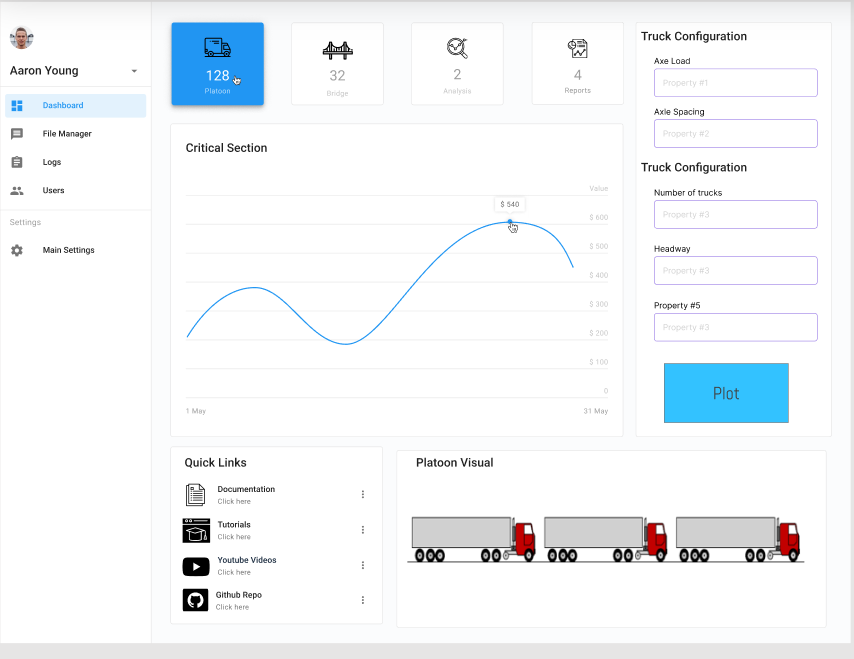
\includegraphics[]{../images/Userinterface-Platoon.PNG}
  \caption{Userinterface Platoon Diagram}
  \label{fig:userinterface-platoon-diagram}
\end{figure}
The screen where the user inputs information related to the truck configuration including the axle load, axle spacing, number of trucks and headway. A visual feedback of the inputted information is given at the bottom of the page to the user for confirmation. The effects of the specified platoon configuration to the critical/concerned section is displayed real-time as a graph in the middle of the screen. \\\\
\begin{figure}[H]
  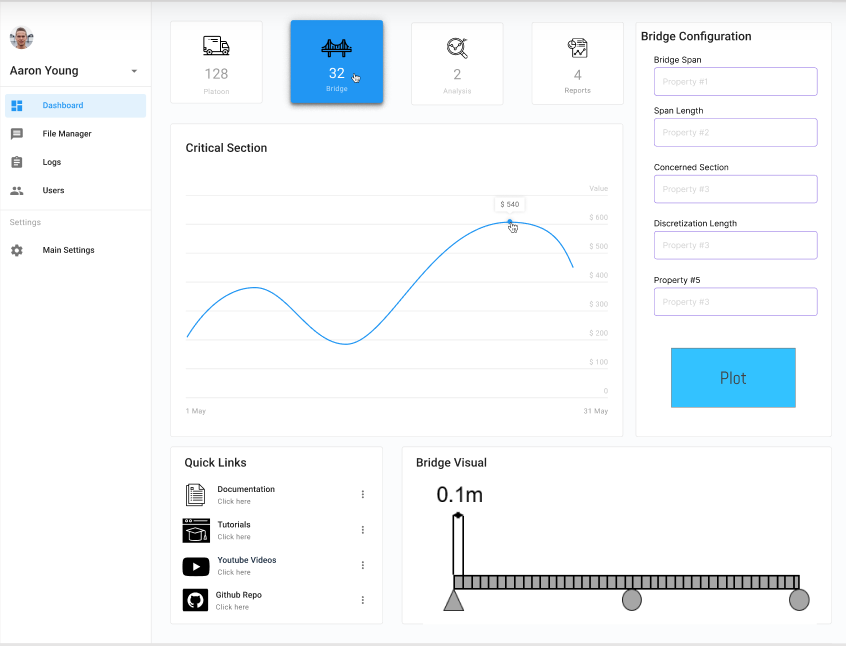
\includegraphics[]{../images/Userinterface-Bridge.PNG}
  \caption{Userinterface Bridge Diagram}
  \label{fig:userinterface-bridge-diagram}
\end{figure}
The screen where the user inputs information related to the Bridge configuration including the bridge span, span length, section of concern and the discretization length. A visual feedback of the inputted information is given at the bottom of the page to the user for confirmation. The effects of the specified bridge configuration to the critical/concerned section is displayed real-time as a graph in the middle of the screen.\\\\
\begin{figure}[H]
  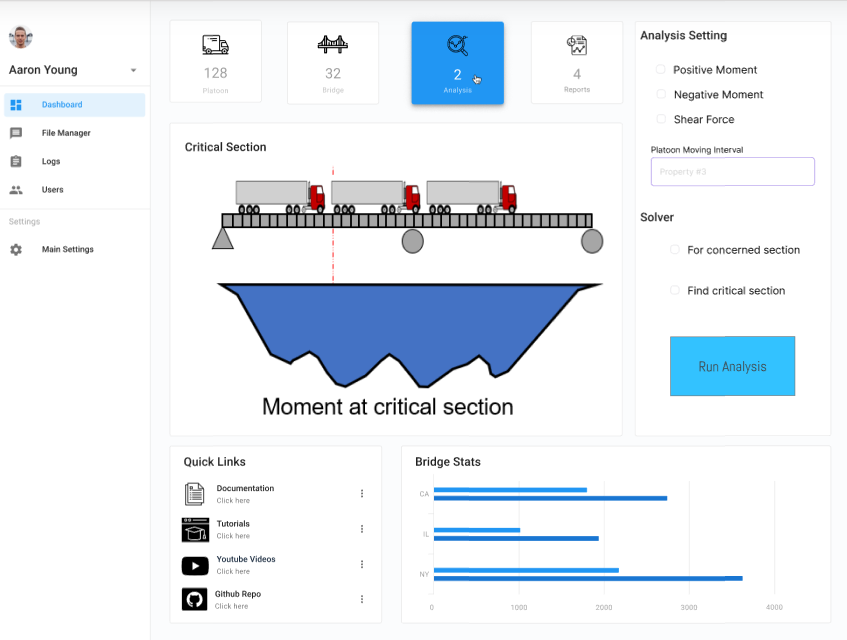
\includegraphics[]{../images/Userinterface-Analysis.PNG}
  \caption{Userinterface Analysis Diagram}
  \label{fig:userinterface-analysis-diagram}
\end{figure}
The screen where the user determines the Analysis setting as well as the the section to be analyzed.\\\\
\begin{figure}[H]
  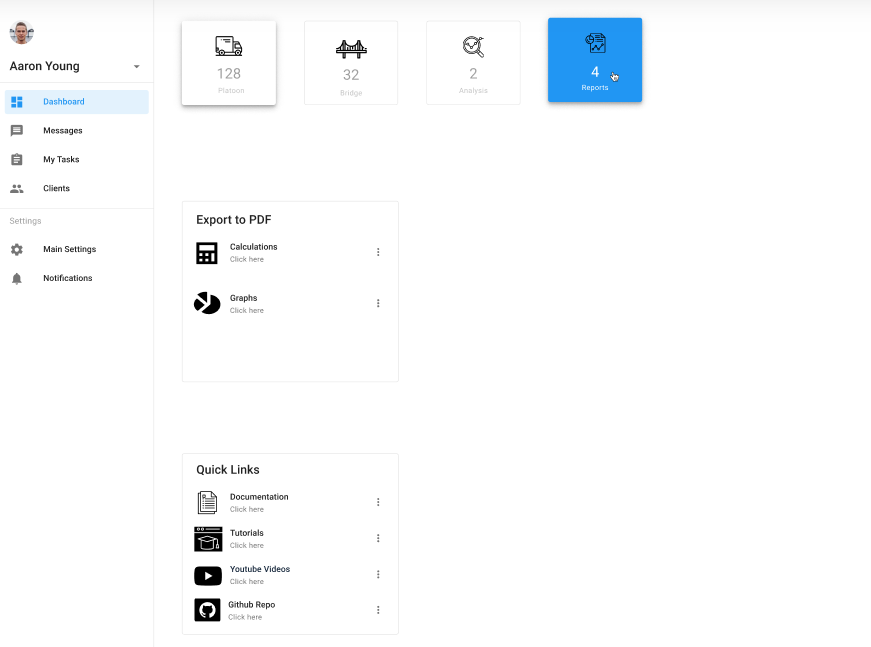
\includegraphics[]{../images/Userinterface-Report.PNG}
  \caption{Userinterface Report Diagram}
  \label{fig:userinterface-report-diagram}
\end{figure}
The screen where the calculations done by the solver and the outputed graphs can be exported to PDF.

\section{Design of Hardware}
N/A

\section{Design of Electrical Components}
N/A

\section{Design of Communication Protocols}

The only communication protocol used by the program is when it communicates with the MATLAB script. This actually uses two protocols: the method names and parameters defined in the MATLAB code, and the functionality implemented by the OS that allows our program to call the MATLAB script. Neither of these communication protocols has been designed by the project team.


\section{Timeline}

\begin{figure}[H]
  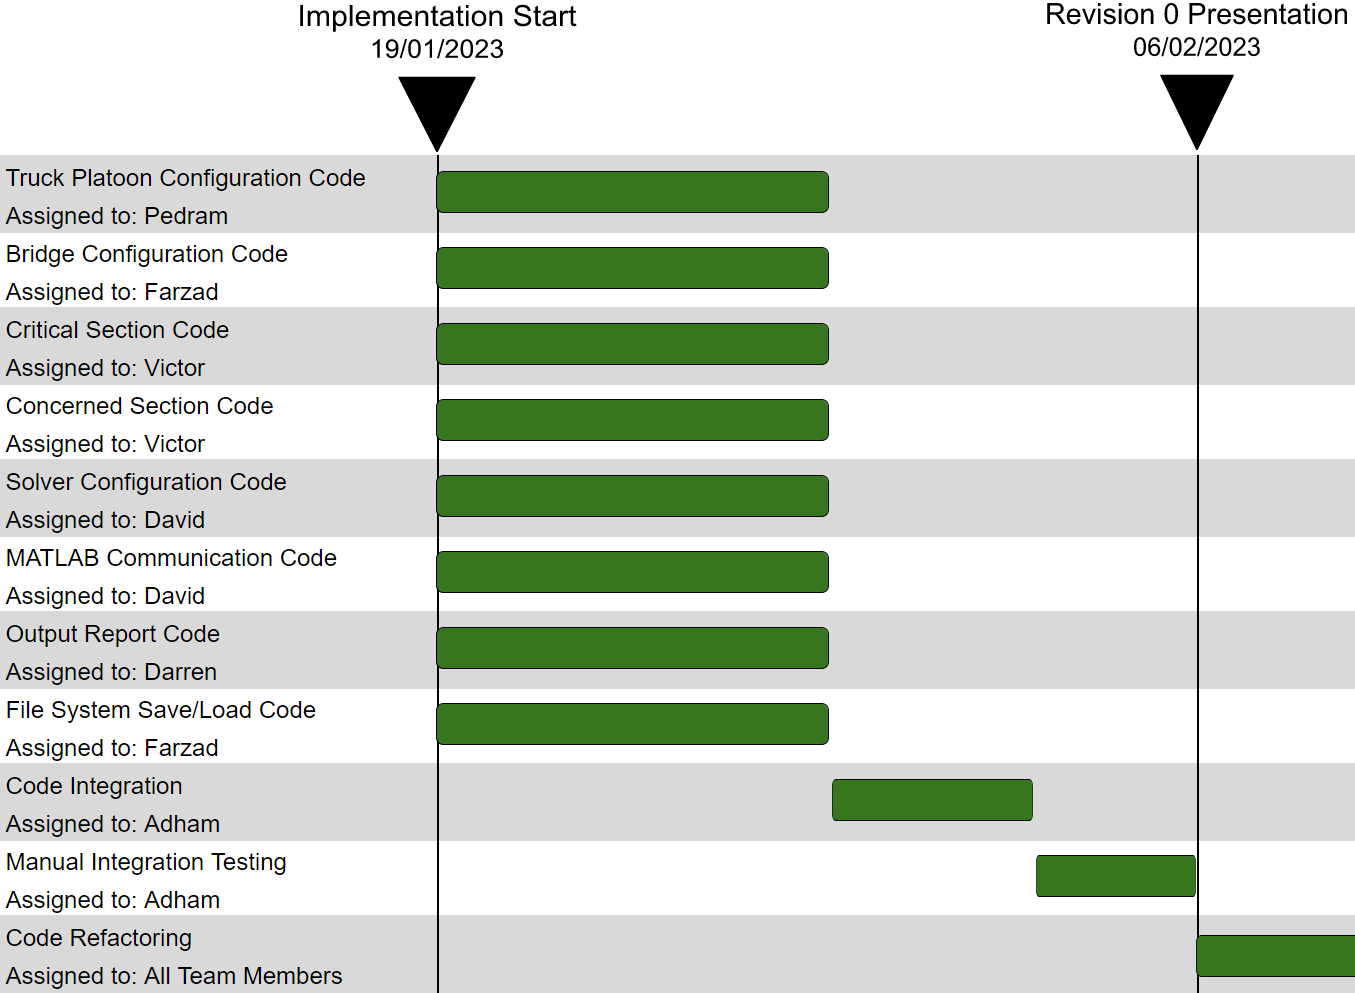
\includegraphics[scale=0.7]{../images/Timeline1.PNG}
  \caption{Project Timeline Section 1}
  \label{fig:timeline1}
\end{figure}

\begin{landscape}
\newpage

\begin{figure}[H]
  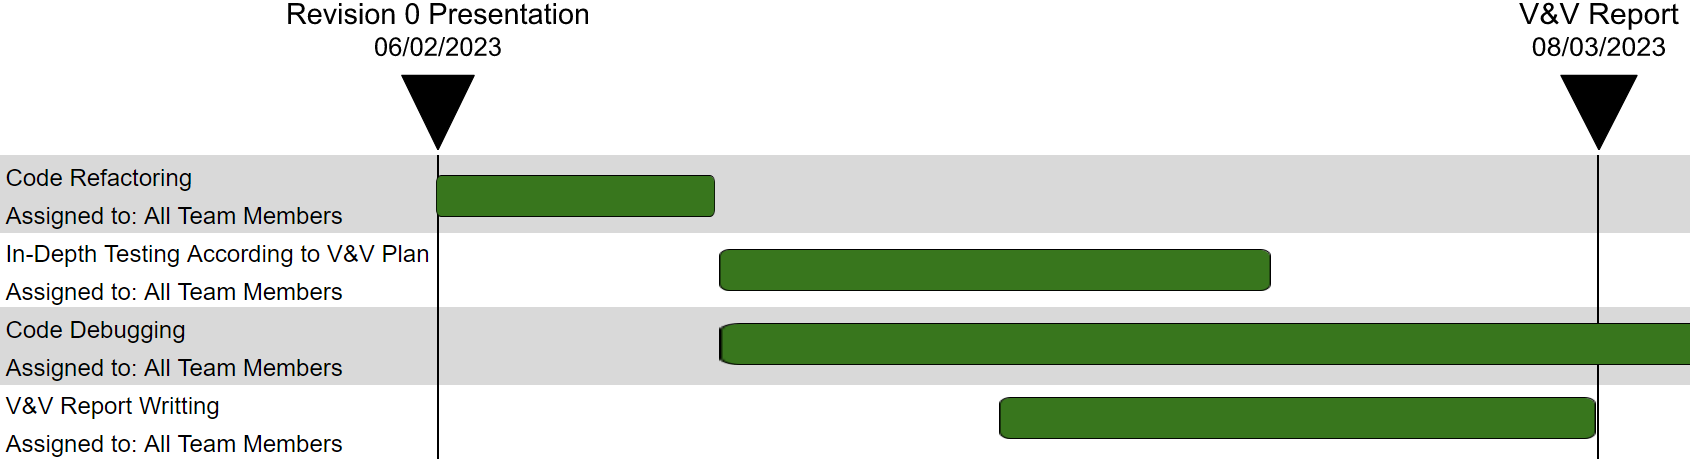
\includegraphics[scale=0.65]{../images/Timeline2.PNG}
  \caption{Project Timeline Section 2}
  \label{fig:timeline2}
\end{figure}

\begin{figure}[H]
  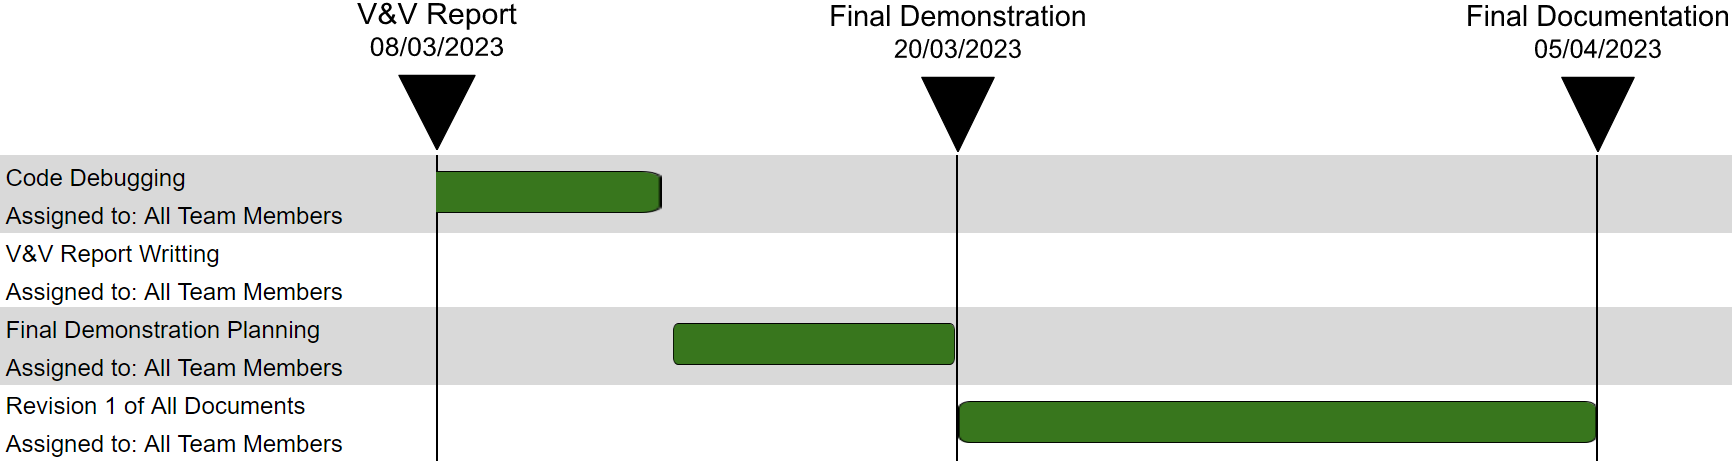
\includegraphics[scale=0.65]{../images/Timeline3.PNG}
  \caption{Project Timeline Section 3}
  \label{fig:timeline3}
\end{figure}

\end{landscape}

% \bibliographystyle {plainnat}
% \bibliography{../../../refs/References}

\newpage{}

\appendix

\section{Interface}

\wss{Include additional information related to the appearance of, and
interaction with, the user interface}

\section{Mechanical Hardware}
N/A
\section{Electrical Components}
N/A
\section{Communication Protocols}
N/A
\section{Reflection}

The information in this section will be used to evaluate the team members on the
graduate attribute of Problem Analysis and Design.  Please answer the following questions:

\begin{enumerate}
  \item What are the limitations of your solution?  Put another way, given
  unlimited resources, what could you do to make the project better? (LO\_ProbSolutions)
  \item Give a brief overview of other design solutions you considered.  What
  are the benefits and tradeoffs of those other designs compared with the chosen
  design?  From all the potential options, why did you select documented design?
  (LO\_Explores)
\end{enumerate}

\end{document}